\chapter{Chapter 1. Introduction}

\section{Space Environment}
\subsection{Near-Earth solar wind}
\subsection{Interplanetary magnetic field}
The interplanetary magnetic field (\gls{IMF}) is the magnetic field of the sun that is carried out in the solar system by the solar wind. The IMF takes the shape of an Archimedean spiral due to the rotation of the sun.

\begin{figure}
    \centering
    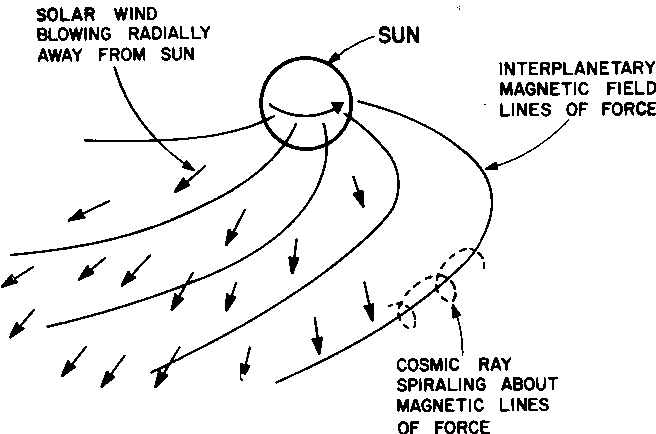
\includegraphics[width=\linewidth]{Figures/IMF.png}
    \caption[Diagram of the interplanetary magnetic field]{The IMF moves away from the sun in an Archimedean spiral.}
    \label{fig:IMF-spiral}
\end{figure}

\subsection{Bow shock}
As a spacecraft traverses near-Earth space, it moves from the solar wind through the different regimes of the terrestrial magnetosphere, the spatial domain of the magnetic-field lines that connect to the Earth \cite{Borovsky:2018}. The magnetosphere presents an obstacle to the flow of the solar wind, and as the solar wind rapidly decelerates from supersonic flow into a subsonic flow, a standing fast shock is formed upstream of Earth \citep{Dimmock:2013}. The plasma is deflected around the magnetosphere as it reaches the bow shock. The bow shock is a collisionless shock that forms from the interaction of the solar wind and Earth's magnetic field. It forms a parabolic boundary around the Earth, with the nose being approximately 15 \gls{RE} in distance in the sunward direction. However, this boundary is constantly moving due to solar wind properties. Many studies have used statistics \citep{Kruparova:2019}, machine learning techniques \citep{Lalti:2022}, or empirical models \citep{chapman_three-dimensional_2003} to identify and locate bow shock crossings of different spacecraft. The interaction of the solar wind with the bow shock can generate magnetic islands and other structures \citep{Karimabadi:2014}, and interaction with the magnetosheath leads wave generation and dissipation, magnetic reconnection, and turbulence \citep{Shaikh:2022}. %As structures and 

\subsection{Magnetosheath}
The magnetosheath is a region of shocked, turbulent, highly magnetized plasma that forms directly downstream of the bow shock. The flow of the solar wind is impeded by the Earth's magnetic field; therefore, the compressed, heated, and turbulent solar wind gets wrapped around Earth's magnetic field. This interface between Earth's terrestrial magnetosphere and the solar wind plays a significant role in the flow of particles across these boundaries. Plasma in the magnetosheath experiences large fluctuations, and \cite{Hadid:2018} estimates that the average energy cascade rate within the magnetosheath is approximately two orders of magnitude larger than the solar wind. The geometry of the bow shock and the interplanetary magnetic field determines the plasma dynamics of the magnetosheath \citep{Yordanova:2020}. Under a quasi-parallel angle of the shock normal ($<45^\circ$), the IMF is connected to the Earth's magnetic field, allowing particles to more easily enter the Earth's terrestrial magnetosphere. One such region which is under a quasi-parallel shock normal is the foreshock region, which is the region in between the last interplanetary field line that connects to the bow shock and the bow shock itself \citep{Karlsson:2021}. In the foreshock region, many solar wind particles are reflected by the bow shock, causing instabilities and other upstream phenomena, which in turn creates intense wave activity \citep{turc_transmission_2023}, such as fast magnetosonic waves \citep{Anderson:1994}. Under a quasi-perpendicular angle of the shock normal ($>45^\circ$), the plasma experiences a sharp decrease in the velocity and sharp increase in the magnitude of the magnetic field. The temperature anisotropy is typically larger in the quasi-perpendicular region, and the quasi-perpendicular region has lower energy flux than the quasi-parallel region \citep{Gurchumelia:2022}. This turbulent layer of plasma is bounded by the magnetopause, which is the outer boundary that separates the solar wind from the magnetosphere. 

\subsection{Magnetopause}
The magnetopause is the boundary at which the solar wind pressure is equal to the dynamic pressure of Earth's magnetic field \citep{Shue:1997}. Because the pressure is not static, the magnetopause boundary moves in relation to the solar wind properties. The standoff distance of the magnetopause nose can be estimated by taking the solar wind ram pressure and setting it equal to the magnetic pressure of Earth's magnetic field. This distance is typically 6-15 $R_E$, based on solar wind conditions \citep{Collado-Vega:2023}. Figure \ref{fig:magnetopause} shows an overview of the bow shock and magnetopause boundaries, as well as a representation of the flow of plasma (black arrows). 

\begin{figure}
    \centering
    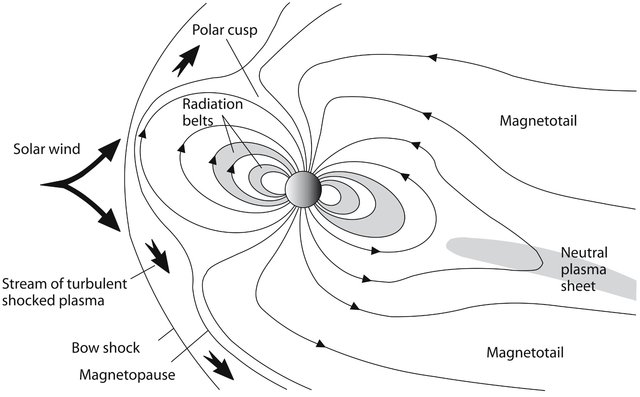
\includegraphics[width=\linewidth]{Figures/The-magnetosphere-is-the-region-where-Earths-magnetic-field-predominates-The_W640.jpg}
    \caption[Diagram of the Earth's magnetopause and magnetic field lines.]{Diagram of the magnetopause and Earth's magnetic field lines \citep{Anderson:2018}. The arrows show the direction of the flow of plasma as it enters the magnetosheath and is wrapped around the magnetosphere. The non-uniform shape of the magnetopause can be seen.}
    \label{fig:magnetopause}
\end{figure}

The magnetopause acts as a sieve, allowing charged particles to enter the magnetosphere. Energetic particles entering the terrestrial magnetosphere leads to geomagnetic activity and has implications for space weather. Positive (negative) ions that drift westward (eastward) contribute to the ring current, which affects the strength of a geomagnetic storm \citep{Williams:1981}. Reconnection of the magnetopause with the IMF injects magnetic flux into the tail region of the magnetosphere \citep{Tsurutani:1990}. Vortices at the edges of the magnetopause, \textit{e.g.} Kelvin-Helmholtz vortices which occur from a shear due to the velocity difference of the magnetosphere and solar wind plasmas across the magnetopause interface \citep{Nykyri:2001}, can also act as a method of two-way transport of energetic particles.

\subsection{Magnetosphere}
The magnetopause is the boundary at which the Earth's magnetic field becomes the dominant magnetic field in the region. This region, the magnetosphere, is highly dynamic due the influx of mass, momentum, and energy from the solar wind. As can be seen in Figure \ref{fig:magnetopause}, the Earth's magnetosphere is a dipole; however, it is by the solar wind from the dayside out to several tens of Earth radii in the nightside \citep{Borovsky:2018}. The inner magnetosphere region is comprised of cold plasma, which rotates with the Earth. This rotation causes the donut-like shape of the plasmasphere \citep{Borovsky:2018}. 

There are currents (due to the change in magnetic field) in the inner magnetosphere: the ring current, Birkeland current, and currents that run along the magnetopause surface boundary, as well as radiation belts. The ring current occurs when charged particles are trapped in the magnetosphere, and the current forms due to the drift of these particles. A decrease in the ring current (Dst index) corresponds to geomagnetic storms. The Birkeland current arises from the flow of electrons along geomagnetic field lines. The Van Allen radiation belts are where energetic particles trapped in the Earth's magnetosphere reside. These radiation belts (inner and outer) pose a hazards to spacecraft in their vicinity, however they do protect the lower altitude from the radiation effects of solar wind and cosmic rays.
% they `bounce' along the field lines (westward for electrons and eastward for ions)

\section{Turbulence \& Coherent structures}
As energy cascades through a system, it is transferred to increasingly smaller scales, and is eventually dissipated. This turbulent process leads to numerous physical effects, including the formation of structures caused by fluctuations in the velocities, magnetic field, and density of plasmas \citep{Matthaeus:2015}. Since these various quantities are transported along the direction of the magnetic field lines, the stagnation of these quantities leads to an accumulation of gradients. Neutral points and points of stagnation therefore play a key role in coherent structure formation \citep{Matthaeus:2015}. Cellularization, which is when relatively relaxed regions separated by strong gradients occur, due to the combined effects of this transport and the concentration of gradients \citep{Matthaeus:2015}. Self-organization such as a cellularization is associated with turbulence, specifically in which one quantity is dissipated while the other quantities are held constant. Rapid relaxation of self-organized cells happens differently for distinct cells: stress accumulates along boundaries with other cells as each region relaxes to a maximal extent. As these boundaries experience higher stress, they become concentrated and form small-scale coherent structures, for example current sheets. Larger scale cells are then formed from the partially relaxed regions. These cells form structures such as flux tubes \citep{Matthaeus:2015}.


\subsection{Interplanetary flux ropes}
In magnetohydrodynamics, the magnetic field geometry influences the direction in which various quantities (energy, plasma quantities, etc.) are transported. When the magnetic field lines are twisted such that they preside in a distinctive tube-like volume with a coherent helical configuration, they are often characterized as a flux rope. Small-scale flux ropes (SFRs) typically exhibit spatial scales $\lesssim$ 0.01 AU and time scales from less than a few minutes to a few hours based on \textit{in situ} spacecraft measurements and analysis in the solar wind near Earth \citep{Cartwright:2010, Feng:2007, Hu:2018}.

\subsection{Alfv\'enic structures}
The helical structure of SFRs leads to high levels of magnetic helicity $H_m$, a measure of twistedness of the field lines. Another quantity that can be used to distinguish magnetic structures is residual energy, $E_r$, which characterizes the imbalance between magnetic and kinetic energy. Flux ropes also exhibit low levels of Alfv\'enicity, the correlation between velocity and magnetic field fluctuations which can be represented by cross helicity $H_c$. Alfv\'enic structures are structures that exhibit high levels of Alfv\'enic characteristics.

%Alfv\'en waves are electromagnetic waves in which ions oscillate along a magnetic field line at the Alfv\'en speed. The restorative force comes from background magnetic field providing an effective tension tension while the inertia comes from the mass of the ions \cite{Alfven:1942}.

These two parameters have been widely adopted as a way to describe the degree of Alfv\'enicity based on time-series analysis. For Alfv\'enic structures, the absolute value of the normalized cross helicity $|\sigma_c|$ is close to 1, and the normalized residual energy $\sigma_r$ is close to 0. For pure Alfv\'en waves, these two quantities are suggested to be 1 and 0, respectively \citep{Bruno:2013}. Flux ropes in the traditional view are supposed to have low Alfv\'enicity, \textit{i.e.}, being static. Considering the crossing of the boundary between the solar wind and the magnetosheath, we adopt a broad definition of SFRs in this study, by including both quasi-static structures and those possessing significant field-aligned flows with modest to high levels of Alfv\'enicity \citep{Chen:2022}.

\subsection{Current sheets}
Alfv\'enic structures, along with current sheets, flux tubes, and/or magnetic flux ropes, occur on a wide range of spatial scales that are increasingly resolved by modern spacecraft measurements \citep{Greco:2018, Pecora:2019, Zheng:2018, Artemyev:2019}.

\section{Objectives}

\section{Organization}

